\documentclass[zh]{assignment}
\ProjectInfos{导波光学}{EE290C}{2020-2021学年第一学期}{课程项目报告\\硅基波导的色散优化和非线性波长转换}{截止时间:2021. 01. 10(周日)}{陈稼霖}{45875852}
\begin{document}

\tableofcontents

\begin{abstract}
    本报告基于文献 \cite{guo2018experimentally},复现其中优化三氧化二铝镀层-二氧化硅包层条形硅基波导色散特性以实现高效率宽带非线性波长转换的过程. 本报告首先介绍利用四波混频实现非线性波长转换的原理和应用,然后分析得到最大化硅基波导非线性波长转换效率和带宽的具体优化目标,最后根据这些目标通过Lumerical仿真,比较了各种结构的硅基波导的色散特性和有效模场面积,优化得到了芯层宽度、镀层厚度等参数的最佳组合,并利用波导四波混频的耦合波方程计算了光场在硅基波导传输过程中各波长转化效率的变化情况.
\end{abstract}

\section{背景介绍}

四波混频效应(four-wave mixing, FWM)是一种三阶非线性光学效应. 该效应是指,非线性介质吸收两个泵浦(pump)光子而被激发,然后回落至基态并发射一对信号(signal)光子和闲频(idler)光子(图 \ref{FWM}(a)). 参与四波混频的四个光子需满足能量守恒定律(图 \ref{FWM}(b)),故有
\begin{align}
    \omega_{p,1}+\omega_{p,2}=\omega_s+\omega_i,
\end{align}
其中 $\omega_{p,1}$,$\omega_{p,2}$ 分别为两个泵浦光子的角频率,$\omega_s$,$\omega_i$ 分别为信号光子和闲频光子的角频率.

不同频率的光场在介质中传输的过程中存在相位失配 \cite{RN158}:一方面,由于介质的色散,不同频率光场在介质中具有不同的传输速度,从而沿着传输方向逐渐分离,在波导中,色散表现为不同频率的光场传输常数的差异,波导色散导致的线性相位失配由传输常数差
\begin{align}
    \Delta\beta=\beta_s+\beta_i-\beta_{p,1}-\beta_{p,2}
\end{align}
来衡量;
另一方面,由于克尔效应(Kerr effect),各频率光场会产生自相位调制(self-phase modulation, SPM)和交叉相位调制(cross-phase modulation, XPM),从而引起非线性相移,通常泵浦光场远强于信号光场和闲频光场,此时克尔效应引起的非线性相位失配近似正比于泵浦光场总功率,即 $\gamma P_p$,其中 $\gamma$ 为非线性系数. 当满足相位匹配(phase matching)条件
\begin{align}
    \label{phase-matching condition}
    \gamma P_p+\Delta\beta=0,
\end{align}
由色散导致的线性相位失配和克尔效应导致的非线性相移抵消,不同频率光场在介质内以相近的速度传输,此时波长转换过程能够持续、有效地进行,四波混频效应最为显著.

\begin{figure}[ht]
    \centering
    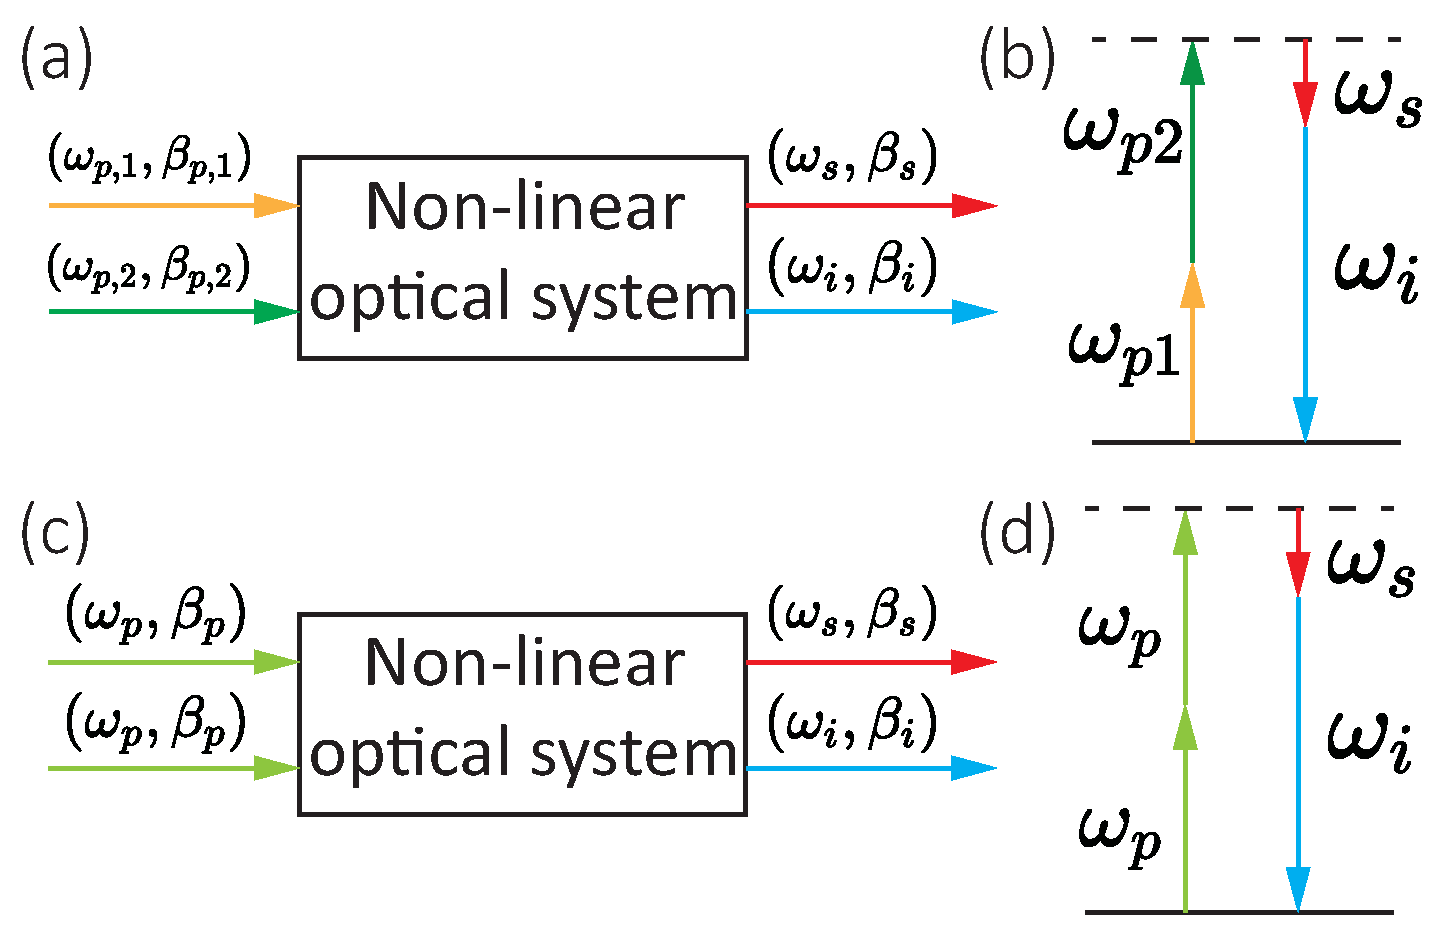
\includegraphics[width=.6\columnwidth]{FWM.eps}
    \caption{(a)(c) 四波混频效应示意图. (b)(d) 能量守恒示意图,其中 (a)(b) --- 非简并四波混频,(c)(d) --- 简并四波混频.}
    \label{FWM}
\end{figure}

根据输入泵浦光频率是否相同,四波混频效应可分为简并(degenerate)四波混频和非简并(non-degenerate)四波混频. 通常情况下,两泵浦光的频率不同,对应的四波混频效应为非简并四波混频效应. 当仅有单一频率的泵浦光输入时,可视为两泵浦光具有相同频率,此时发生的四波混频效应为简并四波混频效应(图 \ref{FWM} (c)),能量守恒(图 \ref{FWM} (d))条件化为
\begin{align}
    2\omega_p=\omega_s+\omega_i,
\end{align}
其中 $\omega_p$ 为泵浦光的角频率.

四波混频效应中,泵浦光、信号光、闲频光通常根据能量进行区分,泵浦光场的能量往往远大于信号光场和闲频光场的能量. 非线性介质除了吸收泵浦光子发射信号光子和闲频光子的过程外,也存在吸收信号光子和闲频光子发射泵浦光子的过程,只不过这种过程相对较弱,实际处理中可忽略不计. 根据实际输入介质的光场频率,四波混频效应还可分为调制不稳定性效应(modulation instability, MI)和布拉格散射效应(Bragg scattering, BS)两种情况. 前者是指,同时输入单一频率的泵浦光和信号光,其中泵浦光场功率远大于信号光场,能量由泵浦光场向信号光场转移从而使信号光场获得参量增益(光学参量放大)并同时从真空噪声中诱导产生稳定的闲频光输出. 在泵浦光场为连续波(continuous wave, CW)的情况下,经过调制编码的信号光场中的时间信息会复制到闲频光场,此即非线性波长转换(non-linear wavelength conversion). 布拉格散射效应则是指同时向非线性介质中输入泵浦光、信号光和闲频光引起的四波混频效应. 泵浦光场能量同时向信号光场和闲频光场转移使信号光场和闲频光场同时获得参量增益.

非线性波长转换,可以将信号光场所载信息复制到闲频光场中,在经典通信领域可用于波分复用(wavelength division multiplexing, WDM)、非线性多点广播(multicasting)等;非线性波长转换还可用于弱相干光子对的产生,是量子通信领域的研究重点之一.

\section{优化目标}

本报告处理的场景为简并四波混频效应的调制不稳定性效应,其参量增益系数定义为
\begin{align}
    \label{gain factor}
    g=\sqrt{-\gamma P_p\Delta\beta+\Delta\beta^2/4},
\end{align}
其中非线性系数
\begin{align}
    \label{non-linear coefficient}
    \gamma=\frac{2\pi n_2}{\lambda A_{\text{eff}}},
\end{align}
$n_2$ 为介质的非线性折射率,$A_{\text{eff}}$ 为光场的有效模场面积. 线性相位失配经泰勒展开并略去高阶项后可近似为
\begin{align}
    \Delta\beta\approx\beta_2(\omega_s-\omega_p)^2,
\end{align}
其中
\begin{align}
    \beta_2=\frac{\partial^2\beta}{\partial\omega^2}.
\end{align}

本报告的最终目标是要最大化非线性波长转换的效率和带宽. 为了最大化非线性波长转换的效率,一要尽可能满足相位匹配条件(式 \eqref{phase-matching condition}),由于非线性相移 $\gamma P_p$ 恒为正值且非线性系数 $\gamma$ 往往很小,因此需要线性相位失配 $\Delta\beta$ 为负且绝对值不能太大,即波导对通信波段的光场呈近零反常色散;二要最大化参量增益系数 $g$(式 \eqref{gain factor}),由于 $\Delta\beta$ 为负,故目标转化为最大化非线性系数 $\gamma$(式 \eqref{non-linear coefficient}),而硅基波导的硅芯非线性折射率$n_2$和通信波段光场的波长 $\lambda$ 均没有太多调节的余地,因此需要最大化光场的有效模场面积 $A_{\text{eff}}$. 在近零反常色散的前提下,为了最大化非线性波长转换的带宽,还需要波导的色散曲线尽可能地平缓. 此外,考虑到加工过程中的误差,波导色散特性对所要调控的参数不能太敏感.

考虑到上述目标,用硅基波导实现非线性波长转换有如下优势:首先,相对其他芯层介质,晶体硅具有相对较大的非线性系数,从而可以实现更高的转换效率;其次,相对其他芯层介质,晶体硅具有较大的折射率,在给定的包层和衬底下可以使用更小的芯层横截面积,从而使得有效模场面积更小,实现更高的转换效率;最后,色散优化高度依赖波导的尺寸,对波导制备、加工工艺的要求较高,而对于硅基波导已具有较为成熟和精度较高的工艺,在工程上更易实现.

\section{仿真过程与结果}

本节基于文献 \cite{guo2018experimentally},针对三氧化二铝镀层-二氧化硅包层条形硅基波导进行优化.

首先,对空气上包层条形硅基波导(图 \ref{Al2O3-Coating-Si-based-Strip-WG-Fig-2} (a))、三氧化二铝镀层条形硅基波导(图 \ref{Al2O3-Coating-Si-based-Strip-WG-Fig-2} (b))、二氧化硅包层条形硅基波导(图 \ref{Al2O3-Coating-Si-based-Strip-WG-Fig-2} (c))、三氧化二铝镀层-二氧化硅包层条形硅基波导(图 \ref{Al2O3-Coating-Si-based-Strip-WG-Fig-2} (d))这四种结构的色散特性进行对比. 四种波导均以二氧化硅为衬底,在 Lumerical 的 MODE 中,设定硅芯高度 $H=250$ nm,三氧化二铝镀层(若有)厚度 $T=50$ nm,根据文献 \cite{boidin2016pulsed} 三氧化二铝镀层折射率为 $1.65$,对四种波导分别用脚本从 $300$ nm 至 $800$ nm 以 $10$ nm 步长遍历硅芯宽度 $W$,对各硅芯宽度 $W$ 分别用 frequency sweep 功能以 $5$ nm 为间隔扫描 $1500$ nm 到 $1600$ nm 波长范围,计算 TE$_0$ 模的群速度 $v_g$ 关于波长的变化关系(仿真模型和脚本见文件 Simulation/Si-Strip-Waveguide-With-Al2O3-Thin-Film-Coating/Fig-2-a-*). 用四次多项式拟合群速度倒数 $v_g^{-1}$ 关于角频率 $\omega$ 的关系,并利用
\begin{align}
    \label{beta-2 calculate}
    \beta_2=\frac{\partial}{\partial\omega}\left(\frac{\partial\beta}{\partial\omega}\right)=\frac{\partial v_g^{-1}}{\partial\omega}
\end{align}
计算 $1560$ nm 波长对应的 $\beta_2$(代码见文件 Simulation/Si-Strip-Waveguide-With-Al2O3-Thin-Film-Coating/Results\\/Fig\_2\_a.m). $1560$ nm 波长下四种波导的 $\beta_2$ 关于硅芯宽度 $W$ 的变化关系如图 \ref{Al2O3-Coating-Si-based-Strip-WG-Fig-2} (e) 所示,与文献 \cite{guo2018experimentally} 中利用 \cite{fallahkhair2008vector} 提出的矢量有限差分方法计算得到的结果(图 \ref{Al2O3-Coating-Si-based-Strip-WG-Fig-2} (f))基本一致:四种波导的 $\beta_2$ 均先随着硅芯宽度 $W$ 的增大从较大的正值(正常色散)骤降为绝对值较小的负值(反常色散),然后随着硅芯宽度 $W$ 的增大缓慢上升至接近 $0$,其中空气上包层条形硅基波导和三氧化二铝镀层硅基波导的 $\beta_2$ 均在硅芯宽度 $W=390$ nm 左右达到极小值,而二氧化硅包层条形硅基波导和三氧化二铝镀层-二氧化硅包层条形硅基波导的 $\beta_2$ 则均在硅芯宽度 $W=460$ nm 左右达到极小值. 相较而言,四种波导结构中,三氧化二铝镀层-二氧化硅包层条形硅基波导的 $\beta_2$ 在 $[390\text{ nm},670\text{ nm}]$ 范围内最符合近零反常色散的目标,且关于硅芯宽度 $W$ 的变化最不敏感.

\begin{figure}[ht]
    \centering
    \includegraphics[width=.6\columnwidth]{Al2O3-Coating-Si-based-Strip-WG-Fig-2.eps}
    \caption{(a) 空气上包层条形硅基波导结构. (b) 三氧化二铝镀层条形硅基波导结构. (c) 二氧化硅包层条形硅基波导结构. (d) 三氧化二铝镀层-二氧化硅包层条形硅基波导结构. (e) 仿真结果:$1560$ nm 波长下四种波导 TE$_0$ 模的 $\beta_2$ 随硅芯宽度 $W$ 的变化关系,其中紫色圆形 --- 空气上包层条形硅基波导,绿色倒三角 --- 三氧化二铝镀层条形硅基波导,红色棱形 --- 二氧化硅包层条形硅基波导结构,蓝色星形 --- 三氧化二铝镀层-二氧化硅包层条形硅基波导,对应文献原图:(f) (文献 \cite{guo2018experimentally} Fig. 2. (a)). (g) 仿真结果:四种波导 TE$_0$ 模的 $\beta_2$ 随波长的变化关系,其中设定空气上包层条形硅基波导(紫色)和三氧化二铝镀层条形硅基波导(绿色)的硅芯宽度 $W=390$ nm,二氧化硅包层条形硅基波导(红色)和三氧化二铝镀层-二氧化硅包层条形硅基波导(蓝色)对应文献原图:(f) (文献 \cite{guo2018experimentally} Fig. 2. (b)).}
    \label{Al2O3-Coating-Si-based-Strip-WG-Fig-2}
\end{figure}

对于四种波导,考察其在通信波段上的色散特性. 为了避免加工过程中的误差对波导色散性能的影响,选择四种波导在图 \ref{Al2O3-Coating-Si-based-Strip-WG-Fig-2} (e)(f) 中的极小值点对应的波导尺寸,即设定空气上包层条形硅基波导和三氧化二铝镀层条形硅基波导硅芯宽度 $W=390$ nm,二氧化硅包层条形硅基波导和三氧化二铝镀层-二氧化硅包层条形硅基波导硅芯宽度 $W=460$ nm,四种波导硅芯高度仍均为 $H=250$ nm. 对四种波导分别用 frequency sweep 功能以 $5$ nm 为间隔扫描 $1450$ nm 到 $1650$ nm 波长范围,计算 TE$_0$ 模的群速度 $v_g$ 关于波长的变化关系(仿真模型见文件 Simulation/Si-Strip-Waveguide-With-Al2O3-Thin-Film-Coating/Fig-2-b-*),并用式 \eqref{beta-2 calculate} 计算得到 $\beta_2$(代码见文件 Simulation/Si-Strip-Waveguide-With-Al2O3-Thin-Film-Coating/Results/Fig\_2\_b.m). 四种波导的 $\beta_2$ 随波长的变化关系如图 \ref{Al2O3-Coating-Si-based-Strip-WG-Fig-2} (g) 所示,与文献 \cite{guo2018experimentally} 中得到的结果(图 \ref{Al2O3-Coating-Si-based-Strip-WG-Fig-2} (h))基本一致:四种波导在所仿真的波段均为反常色散,其中三氧化二铝镀层-二氧化硅包层条形硅基波导的 $\beta_2-$Wavelength 曲线最平缓且最接近 $0$,因此,三氧化二铝镀层-二氧化硅包层条形硅基波导的色散特性最适宜实现高效宽带的非线性波长转换.

接下来选取三氧化二铝镀层-二氧化硅包层条形硅基波导为优化对象,以镀层厚度 $T$ 作为待调控的参数进一步优化其色散特性. 选择镀层厚度 $T=50$ nm,$100$ nm,$150$ nm,$250$ nm,对这四种镀层厚度的三氧化二铝镀层-二氧化硅包层条形硅基波导分别用脚本从 $350$ nm 至 $700$ nm 以 $10$ nm 步长遍历硅芯宽度 $W$,对各硅芯宽度 $W$ 分别用 frequency sweep 功能以 $5$ nm 为间隔扫描 $1500$ nm 到 $1600$ nm 波长范围,计算 TE$_0$ 模的群速度 $v_g$ 关于波长的变化关系(仿真模型和代码见文件 Simulation/Si-Strip-Waveguide-With-Al2O3-Thin-Film-Coating/Fig-3-a-*). 用四次多项式拟合群速度倒数 $v_g^{-1}$ 关于角频率 $\omega$ 的关系并利用式 \eqref{beta-2 calculate} 计算 $1560nm$ 波长对应的 $\beta_2$(代码见文件 Simulation/Si-Strip-Waveguide-With-Al2O3-Thin-Film-Coating/Results/Fig\_3\_a.m). $1560$ nm 波长下不同镀层厚度 $T$ 的三氧化二铝镀层-二氧化硅包层双狭缝条形硅基波导的 $\beta_2$ 随硅芯宽度 $W$ 的变化关系如图 \ref{Al2O3-Coating-Si-based-Strip-WG-Fig-3} (a) 所示,与文献 \cite{guo2018experimentally} 中得到的结果(图 \ref{Al2O3-Coating-Si-based-Strip-WG-Fig-3} (b))基本一致:随着镀层厚度增加,波导厚度满足反常色散的范围更窄,这将导致非线性波长转换的带宽变窄,且曲线的极小值点右移,这意味着曲线极小值对应的波导截面积更大,产生的有效模场面积 $A_{\text{eff}}$ 更大,参量增益系数 $g$ 增大,但同时反常色散段的 $\beta_2$ 更加接近 $0$ 且随硅芯宽度的变化更加平缓,这是有利于提高非线性波长转换效率和带宽的. 因此,在优化过程中应当权衡选择适中的镀层厚度.

\begin{figure}[ht]
    \centering
    \includegraphics[width=.6\columnwidth]{Al2O3-Coating-Si-based-Strip-WG-Fig-3.eps}
    \caption{(a) 仿真结果:$1560$ nm 波长下不同镀层厚度 $T$ 的三氧化二铝镀层-二氧化硅包层条形硅基波导 TE$_0$ 模的 $\beta_2$ 随硅芯宽度 $W$ 的变化关系,其中紫色圆形 --- $T=100$ nm,绿色倒三角 --- $T=150$ nm,红色棱形 --- $T=200$ nm,蓝色星形 --- $T=250$ nm,对应文献原图:(b)(文献 \cite{guo2018experimentally} Fig. 3. (a)). (c) 仿真结果:四种尺寸的三氧化二铝镀层-二氧化硅包层条形硅基波导 TE$_0$ 模的 $\beta_2$ 随波长的变化关系,其中紫色 --- $(W=470\text{ nm},T=100\text{ nm})$,绿色 --- $(W=480\text{ nm},T=150\text{ nm})$,红色 --- $(W=490\text{ nm},T=200\text{ nm})$,蓝色 --- $(W=510\text{ nm},T=250\text{ nm})$,对应文献原图:(d)(文献 \cite{guo2018experimentally} Fig. 3. (b)).}
    \label{Al2O3-Coating-Si-based-Strip-WG-Fig-3}
\end{figure}

在上面仿真的基础上,进一步考察各尺寸波导在通信波段上的色散特性. 为了避免加工过程中的误差对波导色散性能的影响,选择图 \ref{Al2O3-Coating-Si-based-Strip-WG-Fig-3} (a)(b) 各条曲线最低点对应的波导尺寸,即设定$(T=100\text{ nm},W=470\text{ nm})$,$(T=150\text{ nm},W=480\text{ nm})$,$(T=200\text{ nm},W=490\text{ nm})$,$(T=250\text{ nm},W=510\text{nm})$四种尺寸,对四种尺寸的波导分别用 frequency sweep 功能以 $5$ nm 为间隔扫描 $145$ nm 到 $1650$ nm 波长范围,计算 TE$_0$ 模的群速度 $v_g$ 关于波长的变化关系(仿真模型见文件 Simulation/Si-Strip-Waveguide-With-Al2O3-Thin-Film-Coating/Fig-3-b-*)并用式 \eqref{beta-2 calculate} 计算得到 $\beta_2$(代码见文件 Simulation/Si-Strip-Waveguide-With-Al2O3-Thin-Film-Coating/Results/Fig\_3\_b.m). 四种尺寸的波导的 $\beta_2$ 随波长的变化关系如图 \ref{Al2O3-Coating-Si-based-Strip-WG-Fig-3} (c) 所示,与文献 \cite{guo2018experimentally} 中得到的结果(图 \ref{Al2O3-Coating-Si-based-Strip-WG-Fig-3} (d))基本一致:四种尺寸的波导在所仿真的波段均为反常色散,且镀层厚度越大,$\beta_2-W$曲线越接近 $0$.

再来考察镀层厚度对有效模场面积的影响. 设定硅芯宽度 $W=460$ nm,高度 $T=250$ nm,分别对二氧化硅包层条形硅基波导和镀层厚度 $T=50$ nm,$100$ nm, $150$ nm, $200$ nm, $250$ nm 的三氧化二铝镀层-二氧化硅包层条形硅基波导用 frequency sweep 功能以 $10$ nm 为间隔扫描 $1450$ nm 至 $1650$ nm 波长范围,计算 TE$_0$ 模的模场分布 $\bm{E}(x,y)=\hat{x}E_x(x,y)+\hat{y}E_y(x,y)+\hat{z}E_z(x,y)$ 、群折射率 $n_g$ 和波长依赖衰减常数 $\alpha_l$(仿真模型见文件 Simulation/Si-Strip-Waveguide-With-Al2O3-Thin-Film-Coating/Fig-4-a-*),用
\begin{align}
    A_{\text{eff}}=\frac{3}{n_g^2n_c^2}\frac{(\int_Sn_w^2\abs{\bm{E}}^2\,\mathrm{d}S)^2}{\int_C\bm{E}^*\cdot[2\abs{\bm{F}}^2\bm{F}+(\bm{F}\cdot\bm{F})\bm{F}^*]\,\mathrm{d}S^2}
\end{align}
计算有效模场面积(代码见文件 Simulation/Si-Strip-Waveguide-With-Al2O3-Thin-Film-Coating/Results/Fit\_4\_a.m),其中 $n_c$ 为硅芯折射率,$n_w(x,y)$ 为波导截面上折射率分布 \cite{guo2017full}. 各波导有效模场面积随波长的变化关系如图 \ref{Al2O3-Coating-Si-based-Strip-WG-Fig-4} (a),其中有效模场面积随波长和镀层厚度的增大而增大的趋势与文献 \cite{guo2018experimentally} 得到的结果(图 \ref{Al2O3-Coating-Si-based-Strip-WG-Fig-4} (b))基本一致,而二氧化硅包层条形硅基波导与三氧化二铝镀层-二氧化硅包层条形硅基波导的有效模场面积大小关系略有出入,但相差不大,对优化方案没有影响.

\begin{figure}[ht]
    \centering
    \includegraphics[width=.6\columnwidth]{Al2O3-Coating-Si-based-Strip-WG-Fig-4.eps}
    \caption{(a) 各波导 TE$_0$ 模有效模场面积随波长的变化关系,其中虚线 --- 二氧化硅包层条形硅基波导,实线 --- 三氧化二铝镀层-二氧化硅包层条形硅基波导,粉色 --- 镀层厚度 $T=50$ nm,黑色 --- $W=100$ nm,红色 --- $T=150$ nm,绿色 --- $T=200$ nm,蓝色 --- $T=250$ nm,左上角子图为镀层厚度 $T=50$ nm 的三氧化二铝镀层-二氧化硅包层条形硅基波导在 $1560$ nm 波长下 TE$_0$ 模的模场分布,对应文献原图:(b)(文献 \cite{guo2018experimentally} Fig. 4. (a)). (c) 各频率船,对应文献原图:(d)(文献 \cite{guo2018experimentally} Fig. 4. (b)).}
    \label{Al2O3-Coating-Si-based-Strip-WG-Fig-4}
\end{figure}

综合考虑色散特性和有效模场面积,选择硅芯宽度 $W=460$ nm,高度 $H=250$ nm,镀层厚度 $T=50$ nm的三氧化二铝镀层-二氧化硅包层条形硅基波导作为优化的最终方案,通过进一步计算得到该结构波导非线性波长转化效率和带宽以检验优化的效果. 将得到的有效模场面积代入耦合波方程 \cite{guo2017full}
\begin{align}
    \frac{\mathrm{d}A_p}{\mathrm{d}z}=&-\frac{1}{2}\alpha_pA_p+i\gamma_e\abs{A_p}^2A_p,\\
    \frac{\mathrm{d}A_s}{\mathrm{d}z}=&-\frac{1}{2}\alpha_sA_s+2i\gamma_e\abs{A_p}^2A_s+i\gamma_eA_p^2A_i^*e^{-i\Delta\beta z},\\
    \frac{\mathrm{d}A_i}{\mathrm{d}z}=&-\frac{1}{2}\alpha_iA_i+2i\gamma_e\abs{A_p}^2A_i+i\gamma_e\abs{A_p}^2A_i+iA_p^2A_s^*e^{-i\Delta\beta z},
\end{align}
计算泵浦光场、信号光场、闲频光场的归一化幅度 $A_p$,$A_s$,$A_i$在传播场的变化情况,其中非线性系数
\begin{align}
    \gamma_e=\frac{\zeta_e\omega_jn_2}{cA_{\text{eff}}}+\frac{i\zeta_e\beta_T}{2A_{\text{eff}}},
\end{align}
实部来源于克尔效应,虚部来源于双光子吸收(two-photon absorption, TPA),取强度依赖折射因子 $n_2=6\times 10^{-18}\text{m}^2/\text{W}$,双光子吸收系数 $\beta_T=4.5\times 10^{-2}\text{m}/\text{W}$,TE 模的极化系数 $\zeta_{\theta}=1.25$ \cite{tsang2002optical}\cite{moss1989dispersion},各光场总衰减常数为仿真所得波长依赖衰减常数 $\alpha_l$ 和 波长依赖载流子吸收常数之和,
\begin{align}
    \alpha_j=&\alpha_{j,l}+\alpha_{f,j},\\
    \alpha_{f,j}=&6.04\times 10^{-10}\lambda_j^2\frac{\zeta_e\beta_T\abs{A_p}^4\tau}{2\hbar\omega_pA_{\text{eff}}^2},
\end{align}
$j=p,s,i$ 分别对应泵浦光场、信号光场和闲频光场,$\lambda_j$ 为光场波长,$\omega_j$ 为光场角频率,载流子寿命 $\tau=10$ ns,初始条件为输入 $1650$ nm 泵浦光场功率 $P_p(z=0)=\abs{A_p(z=0)}^2=15$ dBm,信号光场功率 $P_s(z=0)=\abs{A_s(z=0)}^2=-10$ dBm. 解得各光场幅度 $A_p(z)$,$A_s(z)$,$A_i(z)$ 后用
\begin{align}
    \eta(z)=\frac{P_i(z)}{P_s(z)}=\frac{\abs{A_i(z)}^2}{\abs{A_s(z)}^2}
\end{align}
计算各波长信号光的非线性波长转化效率在传输方向上的变化(代码见文件 Simulation/Si-Strip-Waveguide-With-Al2O3-Thin-Film-Coating/Results/Fig\_4\_b.m),结果如图 \ref{Al2O3-Coating-Si-based-Strip-WG-Fig-4} (b) 所示,非线性波长转换效率在泵浦光波长($1560$ nm)附近有较为稳定的主瓣,在远离泵浦光波长处的非线性波长转换效率有相对较低且关于泵浦光波长对称的多个旁瓣,在波导中传输 $0.5$ cm 后,主瓣非线性波长转换的效率和带宽均达到稳定值,稳定带宽约 $40$ nm,比文献 \cite{guo2018experimentally} 中得到的 $48$ nm 稳定带宽稍小(图 \ref{Al2O3-Coating-Si-based-Strip-WG-Fig-4} (d)),但均比在文献 \cite{guo2017full} 中用二氧化硅包层条形硅基波导实现的 $36$ nm 带宽有所提升,且整个图像随着传输距离变化的基本趋势相符.

至此,通过比较四种不同结构的条形硅基波导而选出了三氧化二铝镀层-二氧化硅包层条形硅基波导作为最佳波导结构,通过调节其硅芯宽度 $W$ 和镀层厚度 $H$ 两个参数,优化得到了色散特性和 TE$_0$ 模有效模场面积最适宜非线性波长转换的波导尺寸 --- $(W=460\text{ nm},T=50\text{ nm})$,最终实现了较高效率和带宽的非线性波长转换.

\appendix
\bibliographystyle{unsrt}
\addcontentsline{toc}{section}{参考文献}
\bibliography{references}
\end{document}